\documentclass{beamer}
\usepackage{color}
\usepackage{bm}
\usepackage{graphicx}
\usepackage{hyperref}
\usepackage{listings}
\beamertemplatenavigationsymbolsempty
\definecolor{mygreen}{rgb}{0,0.6,0}
\definecolor{mymauve}{rgb}{0.58,0,0.82}
\lstset{ %
  backgroundcolor=\color{white},   % choose the background color; you must add \usepackage{color} or \usepackage{xcolor}
  basicstyle=\footnotesize,        % the size of the fonts that are used for the code
  commentstyle=\color{mygreen},    % comment style
  deletekeywords={...},            % if you want to delete keywords from the given language
  extendedchars=true,              % lets you use non-ASCII characters; for 8-bits encodings only, does not work with UTF-8
  frame=single,                    % adds a frame around the code
  keywordstyle=\color{blue},       % keyword style
  language=Python,                 % the language of the code
  rulecolor=\color{black},         % if not set, the frame-color may be changed on line-breaks within not-black text (e.g. comments (green here))
  showspaces=false,                % show spaces everywhere adding particular underscores; it overrides 'showstringspaces'
  showstringspaces=false,          % don't show spaces in strings
  stringstyle=\color{mymauve},     % string literal style
  title=\lstname                   % show the filename of files included with \lstinputlisting; also try caption instead of title
}
\hypersetup{
    colorlinks=true,
    urlcolor=blue
}

\graphicspath{ {./img/} {./charts/} }


\title{Patchy}
\subtitle{An Alternative to Monkey Patching}
\author{Adam Johnson - me@adamj.eu}
\date{20 September 2015}

\begin{document}


\maketitle


\begin{frame}[fragile]\frametitle{Monkey-patching}

    \begin{itemize}
        \item Modifying objects defined in another module:
    \end{itemize}

    \begin{lstlisting}
In [1]: import sys

In [2]: def explode():
   ...:     print("Boom")
   ...:

In [3]: sys.explode = explode

In [4]: sys.explode()
Boom
    \end{lstlisting}

\end{frame}


\begin{frame}[fragile]\frametitle{Monkey-patching}

    \begin{itemize}
        \item Who has written a monkey patch?
        \item Who has worked on codebase that relied on monkey patching somewhere?
    \end{itemize}

    \begin{center}
        
\includegraphics[width=10cm]{monkey}
    \end{center}

\end{frame}


\begin{frame}[fragile]\frametitle{Situation at YPlan}

    \begin{itemize}
        \item A few monkey-patches on Django to customize things not designed for customization
        \item e.g. changing admin class \texttt{history\_view}, a 35 line
              function, by 1 line:
    \end{itemize}

    \begin{lstlisting}
def history_view(self, request, obj_id, context=None):
    # First check if the user can see this history.
    model = self.model
    obj = get_object_or_404(model, pk=unquote(obj_id))

    # Changed from 'self.has_change_permission':
    if not self.has_view_permission(request, obj):
        raise PermissionDenied

    # ... 30 more lines

from django.contrib.admin import ModelAdmin
ModelAdmin.history_view = history_view
\end{lstlisting}

    % These lines have to be copy/pasted!
    % They prevent future updates to this code from Django from being used in our codebase

\end{frame}


\begin{frame}[fragile]\frametitle{Introducing Patchy}

    \begin{itemize}
        \item \textit{Patch the source of python functions at runtime (not monkey-patching - actual patch-patching)}
    \end{itemize}

    \begin{center}
        
\includegraphics[height=5cm]{patchy-pirate}
    \end{center}

\end{frame}


\begin{frame}[fragile]\frametitle{Patchy}

    \begin{itemize}
        \item Actual patch-patching:
    \end{itemize}

    \begin{lstlisting}
>>> def sample():
...    return 1
>>> sample()
1
>>> patchy.patch(sample, """\
...     @@ -1,2 +1,2 @@
...      def sample():
...     -    return 1
...     +    return 9001
...     """)
>>> sample()
9001
    \end{lstlisting}

\end{frame}


\begin{frame}[fragile]\frametitle{Patchy}

    \begin{itemize}
        \item People like 'whut?'
    \end{itemize}

    \begin{center}
        
\includegraphics[width=10cm]{jackie-chan-whut}
    \end{center}

\end{frame}


\begin{frame}[fragile]\frametitle{Admin patch}

    \begin{lstlisting}
from django.contrib.admin.options import ModelAdmin

patchy.patch(ModelAdmin.history_view, """\
@@ -5,7 +5,7 @@ def history_view(self, request, object_id, extra_context=None):
     model = self.model
     obj = get_object_or_404(self.get_queryset(request), pk=unquote(object_id))

-    if not self.has_change_permission(request, obj):
+    if not self.has_view_permission(request, obj):
         raise PermissionDenied

     # Then get the history for this object.
""")
    \end{lstlisting}

    \begin{itemize}
        \item Expresses the change in code rather than a comment
        \item More robust - only the lines around the change are needed
    \end{itemize}

\end{frame}


\begin{frame}[fragile]\frametitle{How it work?}

    \begin{center}
        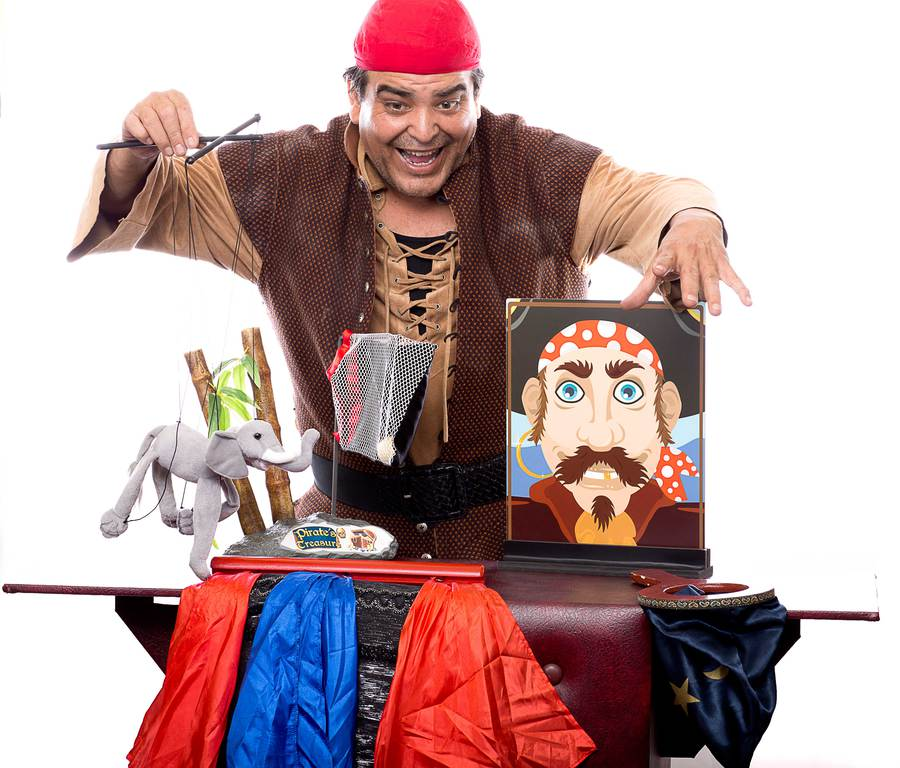
\includegraphics[width=7cm]{magical-pirate}
    \end{center}

    \begin{itemize}
        \item Magic.
    \end{itemize}

\end{frame}


\begin{frame}[fragile]\frametitle{Thank you}

    \begin{center}
        
\includegraphics[width=10cm]{barbossa}
    \end{center}

    \begin{itemize}
        \item \url{github.com/adamchainz/patchy}
        \item \url{me@adamj.eu}
    \end{itemize}

\end{frame}


\end{document}
